\chapter{Additional Studies in Progress}
\label{app:studies_in_progress}

This appendix collects two robustness studies assembled from the finished
result files recovered from Oscar.  Availability is uneven across the
sweep grids, so each table retains dashes wherever no finished result
files were present in the recovered snapshot.

% ======================================================================
\section{Physical inductive biases}
\label{app:pipeline_fixes}
% ======================================================================

Section~\ref{sec:pipeline_fixes} describes six physical inductive biases
in full; a compact summary is reproduced here for self-contained
reference.

\begin{enumerate}[nosep]

  \item \textbf{Centred flux estimation.}
    The KDE flux estimator subtracts the domain-mean flux from each snapshot
    before convolution, preventing a spurious DC offset from aliasing into
    the linear drag coefficient.

  \item \textbf{Biharmonic operator removal.}
    The biharmonic ($\nabla^4$) library term was removed: it is not part of
    the expected mean-field structure and in trial runs absorbed energy from
    the viscous term, degrading interpretability.

  \item \textbf{Temporal test-function width floor.}
    The temporal support is floored at $\ell_t \geq 7$ grid points to prevent
    the width optimiser from collapsing the weak-form integral to a pointwise
    residual.

  \item \textbf{Sign constraints on post-fit coefficients.}
    After each MSTLS solve, coefficients whose physical sign is known
    \emph{a priori} (e.g.\ viscous terms must be non-positive) are checked;
    sign-violating survivors are zeroed and the fit re-solved.

  \item \textbf{Coefficient magnitude cap.}
    Retained coefficients exceeding $|c|>5.0$ are removed, guarding against
    inflation from near-singular library matrices.

  \item \textbf{Regime-aware library construction.}
    The \cv{forces.enabled} flag controls whether Morse potential terms enter
    the candidate library; for pure-Vicsek regimes the Morse columns are
    automatically excluded.

\end{enumerate}

% ======================================================================
\section{Noise robustness}
\label{app:noise_robustness}
% ======================================================================

The primary question is whether the \emph{same mechanisms remain
identifiable} under varying noise, rather than whether weak-form $R^2$
degrades.  We run the full pipeline at five noise levels for each of four
regimes: gas ($\eta\in\{0.15, 0.50, 1.00, 1.50, 2.00\}$, native
$\eta{=}1.5$), blackhole ($\eta\in\{0.05, 0.15, 0.50, 1.00, 1.50\}$,
native $\eta{=}0.15$), supernova ($\eta\in\{0.05, 0.15, 0.50, 1.00,
1.50\}$, native $\eta{=}0.15$), and crystal
($\eta\in\{0.05, 0.10, 0.50, 1.00, 1.50\}$, native $\eta{=}0.10$).
Recovered result files populate 16 of the 20 WSINDy rows and 6 of the 20
companion ROM rows; the remaining cells are left as dashes rather than
being inferred.  Where available, the weak-form $R^2$ and companion MVAR
and LSTM forecast quality are reported in
Table~\ref{tab:noise_sweep_forecast}.

\begin{table}[ht]
\centering
\caption{Noise-sweep forecast $R^2$ (mean over four IC families).
WSINDy $R^2_{\mathrm{wf},\rho}$ reports the weak-form fit on the density
field; dashes indicate that no finished result files were recovered for
that cell.
Native noise levels are marked with~$\star$.
All entries use a single random seed; seed-to-seed variation has not yet been quantified.}
\label{tab:noise_sweep_forecast}
\renewcommand{\arraystretch}{0.92}
\small
\begin{tabular}{llccc}
\toprule
\textbf{Regime} & $\boldsymbol{\eta}$ & \textbf{MVAR} $R^2$ & \textbf{LSTM} $R^2$ & \textbf{WSINDy} $R^2_{\mathrm{wf},\rho}$ \\
\midrule
Gas & 0.15 & --- & --- & --- \\
Gas & 0.50 & 0.993 & 0.972 & 0.9997 \\
Gas & 1.00 & --- & --- & 0.9998 \\
Gas & 1.50$\star$ & 0.994 & 0.977 & 0.9998 \\
Gas & 2.00 & 0.994 & 0.806 & 0.9998 \\
\midrule
Blackhole & 0.05 & 0.994 & 0.988 & --- \\
Blackhole & 0.15$\star$ & 0.986 & 0.966 & --- \\
Blackhole & 0.50 & --- & --- & 0.9996 \\
Blackhole & 1.00 & 0.983 & 0.125 & 0.9997 \\
Blackhole & 1.50 & --- & --- & 0.9998 \\
\midrule
Supernova & 0.05 & --- & --- & 0.9998 \\
Supernova & 0.15$\star$ & --- & --- & 0.9998 \\
Supernova & 0.50 & --- & --- & --- \\
Supernova & 1.00 & --- & --- & 0.9989 \\
Supernova & 1.50 & --- & --- & 0.9982 \\
\midrule
Crystal & 0.05 & --- & --- & 0.9999 \\
Crystal & 0.10$\star$ & --- & --- & 0.9999 \\
Crystal & 0.50 & --- & --- & 0.9999 \\
Crystal & 1.00 & --- & --- & 0.9999 \\
Crystal & 1.50 & --- & --- & 0.9999 \\
\bottomrule
\end{tabular}

\end{table}

Within the recovered ROM subset (gas $\eta\in\{0.50,1.50,2.00\}$ and
blackhole $\eta\in\{0.05,0.15,1.00\}$), MVAR remains strong
($R^2 \geq 0.983$), while LSTM is more variable and drops sharply at
blackhole $\eta{=}1.0$, consistent with the distribution-shift
sensitivity discussed in Section~\ref{sec:ch7_lstm_modes}.  No
companion ROM forecasts were recovered for the supernova or crystal
sweeps, so those rows remain identification-only in
Table~\ref{tab:noise_sweep_forecast}.

WSINDy identification is recovered for gas at four noise levels,
blackhole at three, supernova at four, and crystal at all five; the
missing WSINDy rows are gas $\eta{=}0.15$, blackhole
$\eta\in\{0.05,0.15\}$, and supernova $\eta{=}0.50$.  Wherever the
WSINDy runs finished, the continuity backbone
$\nabla\cdot\mathbf{p}\approx -1$ is retained and the density weak-form
fit remains near unity.  The sole visible degradation appears in the
supernova regime, where $R^2_{\mathrm{wf},\rho}$ drops from $0.9998$
at the native level ($\eta{=}0.15$) to $0.9982$ at $\eta{=}1.50$; all
other regimes remain above $0.9996$
(Figure~\ref{fig:noise_coeff_stability}).

\begin{figure}[ht]
\centering
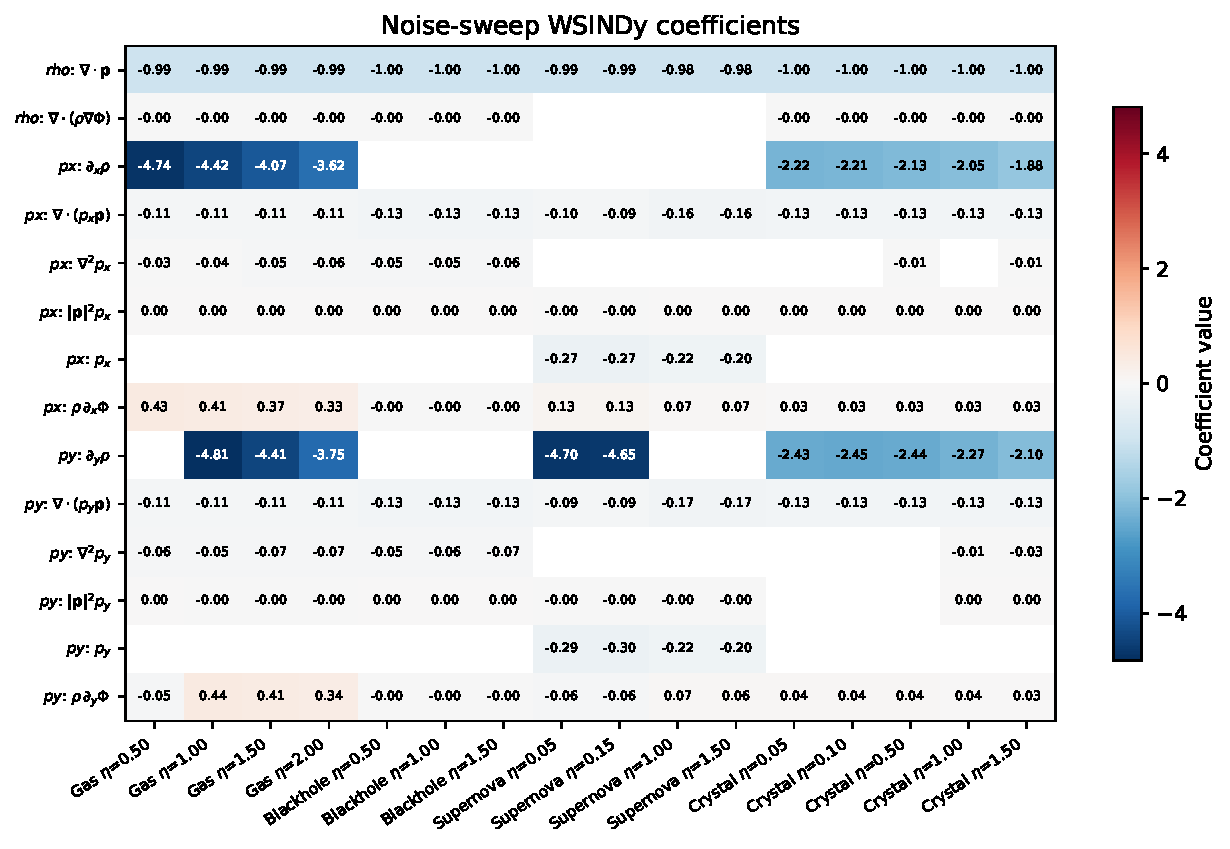
\includegraphics[width=0.82\textwidth]{../Thesis_Figures/noise_coeff_stability.pdf}
\caption{Noise-sweep WSINDy coefficient stability.
Rows correspond to candidate library terms; columns to the
regime--noise configurations recovered from Oscar.
White cells indicate terms absent from the
active set.  The continuity backbone $\nabla\cdot\mathbf{p}\approx -1$
is stable wherever the WSINDy noise runs finished.}
\label{fig:noise_coeff_stability}
\end{figure}

% ======================================================================
\section{Convergence in the number of particles}
\label{app:n_convergence}
% ======================================================================

To verify that the WSINDy-recovered PDEs represent a genuine mean-field
limit, we repeat the pure Vicsek identification at
$N\in\{50, 100, 200, 300, 500, 1000\}$.
Table~\ref{tab:n_convergence_forecast} reports the
companion MVAR and LSTM forecast quality alongside the WSINDy weak-form
$R^2$.  Finished result files are available only for
$N{=}50,100,200,300$; the $N{=}500$ and $N{=}1000$ rows remain blank in
the recovered appendix snapshot.  At all four completed particle counts,
WSINDy recovers $R^2_{\text{wf},\rho}\geq 0.9999$ with a consistent
active set of $|\mathcal{A}|{=}5$ terms (one for $\rho$, two each for
$p_x$ and $p_y$); the reported $R^2_{\text{wf},p}$ values use the
$p_x$ equation, with $p_y$ showing comparable fits in all completed
runs.  Momentum fit ranges from $R^2_{\text{wf},p}{=}0.80$
to~$0.85$, suggesting the mean-field limit is well-approximated even at
moderate particle counts.

\begin{table}[ht]
\centering
\caption{$N$-convergence forecast $R^2$ for pure Vicsek (mean over four
IC families).  MVAR is stable across $N$; LSTM degrades at larger $N$,
possibly due to increased latent dimensionality.  WSINDy weak-form
$R^2_{\mathrm{wf},\rho}\geq 0.9999$ at all completed particle counts;
momentum fit $R^2_{\mathrm{wf},p}$ is in the $0.80$--$0.85$ range,
consistent with the main-text pure Vicsek result ($R^2_{\mathrm{wf},p}{=}0.82$).
Dashes indicate that no finished result files were recovered for that row.}
\label{tab:n_convergence_forecast}
\renewcommand{\arraystretch}{0.92}
\small
\begin{tabular}{rccccc}
\toprule
$N$ & \textbf{MVAR} $R^2$ & \textbf{LSTM} $R^2$ & \textbf{MVAR} $R^2$ (Gaussian IC) & \textbf{WSINDy} $R^2_{\mathrm{wf},\rho}$ & \textbf{WSINDy} $R^2_{\mathrm{wf},p}$ \\
\midrule
50 & 0.635 & 0.229 & 0.982 & 0.9999 & 0.801 \\
100 & 0.542 & 0.085 & 0.992 & 1.0000 & 0.827 \\
200 & 0.647 & $-0.794$ & 0.995 & 1.0000 & 0.849 \\
300 & 0.653 & $-0.914$ & 0.992 & 1.0000 & 0.834 \\
500 & --- & --- & --- & --- & --- \\
1000 & --- & --- & --- & --- & --- \\
\bottomrule
\end{tabular}

\end{table}

MVAR $R^2$ is stable at $0.54$--$0.65$ across the tested range and
reaches $R^2 > 0.98$ on the Gaussian IC family at all particle counts,
indicating that the forecast ceiling is limited by IC diversity rather
than particle number.  LSTM forecast quality degrades from $R^2{=}0.23$
at $N{=}50$ to $R^2{=}-0.91$ at $N{=}300$, reflecting sensitivity to
the growing latent state dimension.  No finished result files were
recovered for $N{=}500$ or $N{=}1000$, so the appendix cannot yet say
whether those trends continue at larger particle counts.

\begin{figure}[ht]
\centering
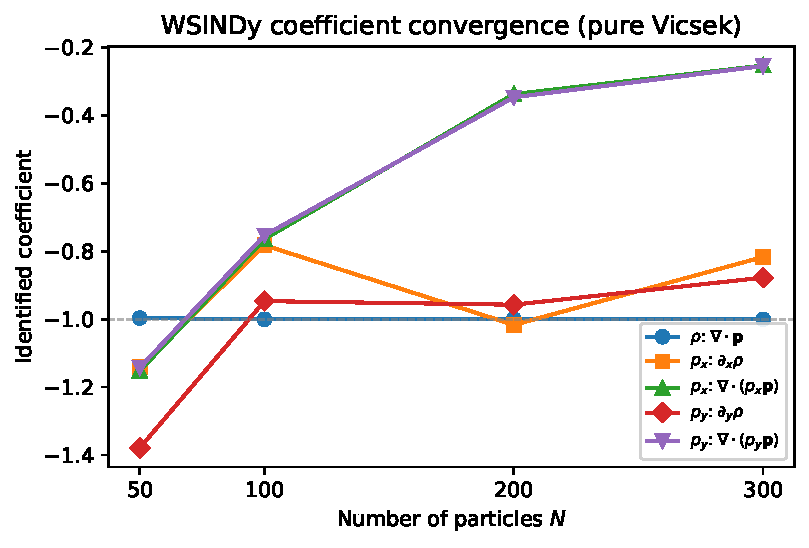
\includegraphics[width=0.78\textwidth]{../Thesis_Figures/n_convergence_coefficients.pdf}
\caption{$N$-convergence of WSINDy-identified coefficients for the
pure Vicsek regime.  Each curve tracks a single coefficient across
$N\in\{50, 100, 200, 300, 500, 1000\}$; gaps indicate unfinished rows.
The continuity coefficient
$\nabla\cdot\mathbf{p}$ (blue) converges to $-1$ at all particle counts;
the momentum pressure and advection terms show larger variation.}
\label{fig:n_convergence_coefficients}
\end{figure}
